\documentclass[tikz,border=8pt]{standalone}
\usepackage{tikz}
\usetikzlibrary{arrows.meta,calc}

\definecolor{primary}{HTML}{143264}
\definecolor{secondary}{HTML}{8C281E}
\definecolor{tealcol}{HTML}{117A65}
\definecolor{orangecol}{HTML}{C77C02}
\definecolor{purplecol}{HTML}{6A3D9A}

\begin{document}
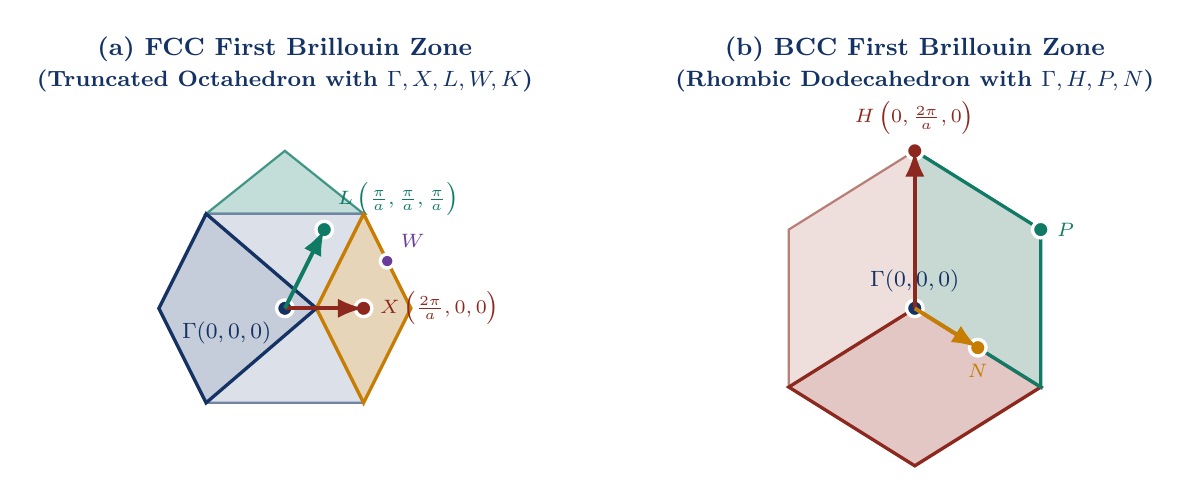
\begin{tikzpicture}[>=Latex]

  % Subfigure (a): FCC 1st Brillouin Zone (Truncated Octahedron)
  \begin{scope}[shift={(0,0)}]
    \node[align=center, font=\bfseries\small, text=primary] at (3.0, 5.5) 
      {(a) FCC First Brillouin Zone\\ \footnotesize (Truncated Octahedron with $\Gamma, X, L, W, K$)};

    \coordinate (Gamma) at (3.0, 2.4);

    \fill[tealcol!25, draw=tealcol!80, thick] (2.0, 3.6) -- (3.0, 4.4) -- (4.0, 3.6) -- cycle;
    \fill[primary!15, draw=primary!60, thick] 
      (1.4, 2.4) -- (2.0, 3.6) -- (4.0, 3.6) -- (4.6, 2.4) -- (4.0, 1.2) -- (2.0, 1.2) -- cycle;

    \fill[orangecol!35, draw=orangecol, very thick, fill opacity=0.7] 
      (4.0, 3.6) -- (4.6, 2.4) -- (4.0, 1.2) -- (3.4, 2.4) -- cycle;

    \fill[primary!30, draw=primary, very thick, fill opacity=0.6] 
      (1.4, 2.4) -- (2.0, 3.6) -- (3.4, 2.4) -- (2.0, 1.2) -- cycle;

    \filldraw[fill=primary, draw=white, very thick] (Gamma) circle (3pt) node[below left=1pt, font=\footnotesize\bfseries, primary] {$\Gamma(0,0,0)$};

    \coordinate (X) at (4.0, 2.4);
    \filldraw[fill=secondary, draw=white, very thick] (X) circle (3pt) node[right=2pt, font=\scriptsize\bfseries, secondary] {$X\left(\frac{2\pi}{a},0,0\right)$};

    \coordinate (L) at (3.5, 3.4);
    \filldraw[fill=tealcol, draw=white, very thick] (L) circle (3pt) node[above right=1pt, font=\scriptsize\bfseries, tealcol] {$L\left(\frac{\pi}{a},\frac{\pi}{a},\frac{\pi}{a}\right)$};

    \coordinate (W) at (4.3, 3.0);
    \filldraw[fill=purplecol, draw=white, very thick] (W) circle (2.5pt) node[above right=1pt, font=\scriptsize\bfseries, purplecol] {$W$};

    \draw[->, line width=1.4pt, secondary] (Gamma) -- (X);
    \draw[->, line width=1.4pt, tealcol] (Gamma) -- (L);
  \end{scope}

  % Subfigure (b): BCC 1st Brillouin Zone (Rhombic Dodecahedron)
  \begin{scope}[shift={(8.0,0)}]
    \node[align=center, font=\bfseries\small, text=primary] at (3.0, 5.5) 
      {(b) BCC First Brillouin Zone\\ \footnotesize (Rhombic Dodecahedron with $\Gamma, H, P, N$)};

    \coordinate (GammaB) at (3.0, 2.4);

    \fill[secondary!15, draw=secondary!60, thick] 
      (3.0, 0.4) -- (4.6, 1.4) -- (4.6, 3.4) -- (3.0, 4.4) -- (1.4, 3.4) -- (1.4, 1.4) -- cycle;
    
    \fill[secondary!30, draw=secondary, very thick, fill opacity=0.7]
      (3.0, 0.4) -- (4.6, 1.4) -- (3.0, 2.4) -- (1.4, 1.4) -- cycle;

    \fill[tealcol!30, draw=tealcol, very thick, fill opacity=0.7]
      (3.0, 2.4) -- (4.6, 1.4) -- (4.6, 3.4) -- (3.0, 4.4) -- cycle;

    \filldraw[fill=primary, draw=white, very thick] (GammaB) circle (3pt) node[above=2pt, font=\footnotesize\bfseries, primary] {$\Gamma(0,0,0)$};
    
    \coordinate (H) at (3.0, 4.4);
    \filldraw[fill=secondary, draw=white, very thick] (H) circle (3pt) node[above=2pt, font=\scriptsize\bfseries, secondary] {$H\left(0,\frac{2\pi}{a},0\right)$};

    \coordinate (P) at (4.6, 3.4);
    \filldraw[fill=tealcol, draw=white, very thick] (P) circle (3pt) node[right=2pt, font=\scriptsize\bfseries, tealcol] {$P$};

    \coordinate (N) at (3.8, 1.9);
    \filldraw[fill=orangecol, draw=white, very thick] (N) circle (3pt) node[below=2pt, font=\scriptsize\bfseries, orangecol] {$N$};

    \draw[->, line width=1.4pt, secondary] (GammaB) -- (H);
    \draw[->, line width=1.4pt, orangecol] (GammaB) -- (N);
  \end{scope}

\end{tikzpicture}
\end{document}
